rate limiting was one interesting aspect for security, as it's a way to prevent the
server from being flooded with requests. As it could stop DDOS attacks, brute force
attacks, and any other kind of attack that would require sending lot of request from 
the same IP or same user.

For the rate limiting, as we were using already a Spring backend we had a couple options
to choose from the first one was Bucket4j, which is a rate limiter that relies on token
bucket algorithm which approaches rate limiting through putting a number of tokens in a
bucket then whenever the consume or client tries to use a service it has to consume one
or more tokens from the bucket until they are depleted then the client is blocked \cite{b4j},
the bucket is then assigned to a key which could be a user, IP address or API key ...

The second option was to use Resilience4j, which relies on creating cycles where each cycle
has a number of allowed permissions and refreshes in the beginning of each cycle\cite{r4j}, which
allows the handling of the rate limiting in a epoch fashion but it was not easy to
implement for the case of a distributed backend and not worth the trouble to adapt it
with a caching system within the Redis Database to do so, as it relied heavily on
single machines threads for the handling it does.

\begin{figure}[!ht]
    \centering
    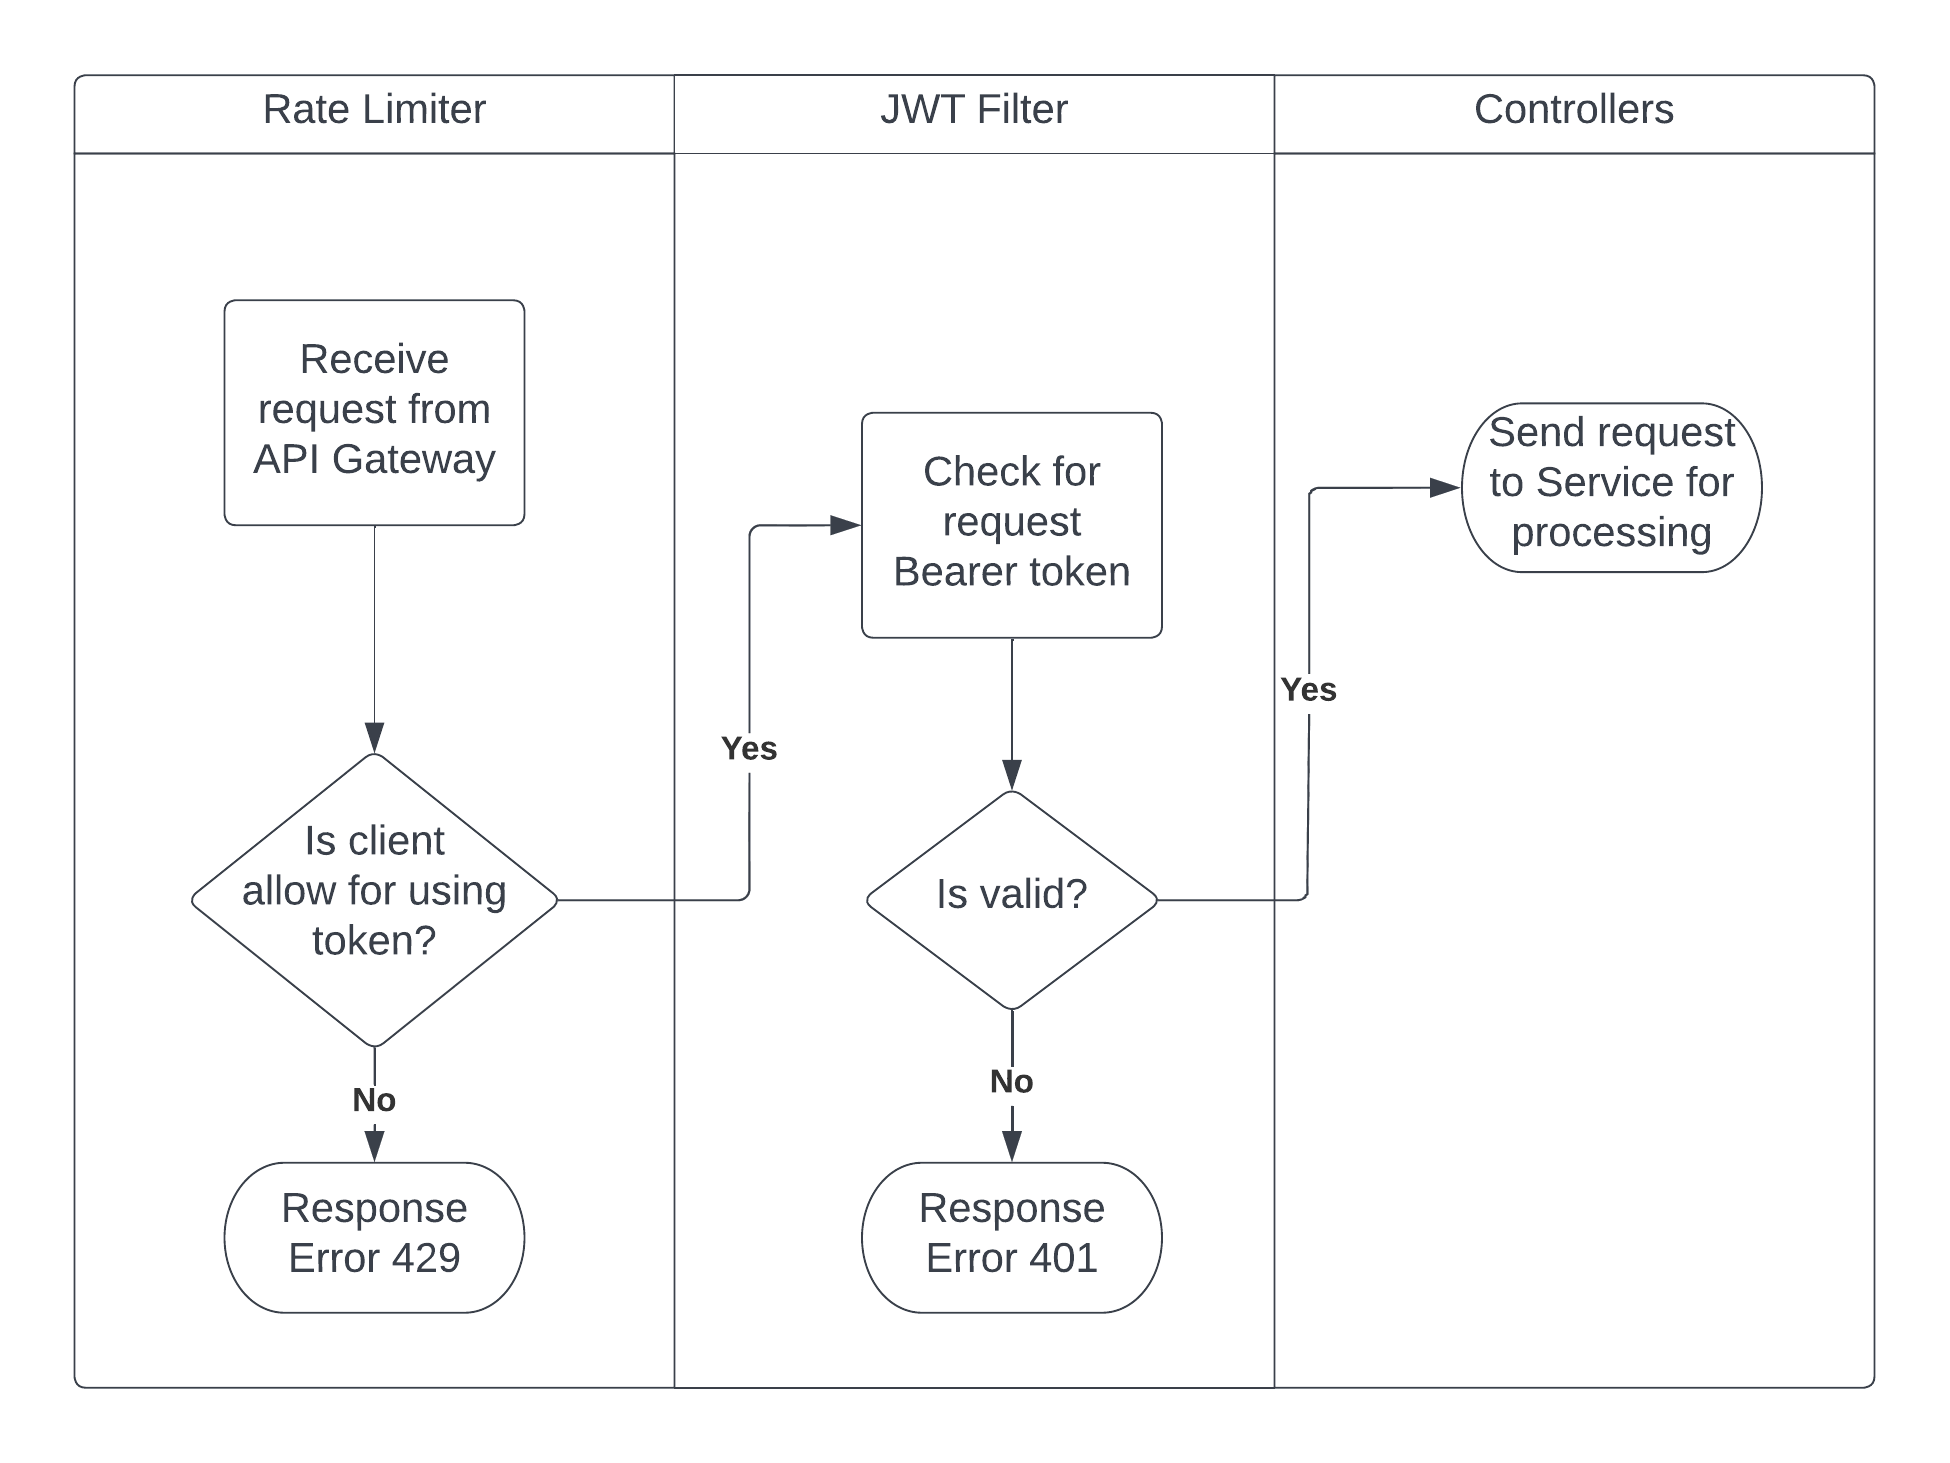
\includegraphics[width=0.9\textwidth]{images/Flow chart b4j.png}
    \caption{\footnotesize{Backend Gateway - Process}}
    \label{fig:b4j}
\end{figure}

So we went with the former, which was implemented as a filter within the API gateway
in the Spring backend as shown figure \ref{fig:b4j}, which is a pretty straight forward:
\begin{itemize}
    \item A request is sent by the client, which is then sent to the backend.
    \item The request gets intercepted by the rate limiter on the filter layer
    \item The request is then either accepted or rejected depending on
        the number of tokens in the bucket:
        \begin {itemize}
            \item If the bucket contains a token, the request is sent to the authorizaiton
                filter.
            \item If the bucket has no tokens left the request is rejected and the client
                receives a 429 error, which matches "Too Many Requests".
        \end {itemize}
\end{itemize}

So the now the handling of services within the Java Spring backend required the passage
from API rate limiter which consisted of giving a token to the client before allowing
the request to be processed, and this requests were by default capped to a certain number
that could be modified through the configuration file of the server.

Now with the basic handling in hand, we opt for the implementation of the rate limiter
which was done in two ways which are displayed in \ref{fig:ratelimiting_flow}, the first
was to have a bucket for each user using their JWT token, and the second was to have a bucket
for each IP address.

\begin{figure}[!ht]
    \centering
    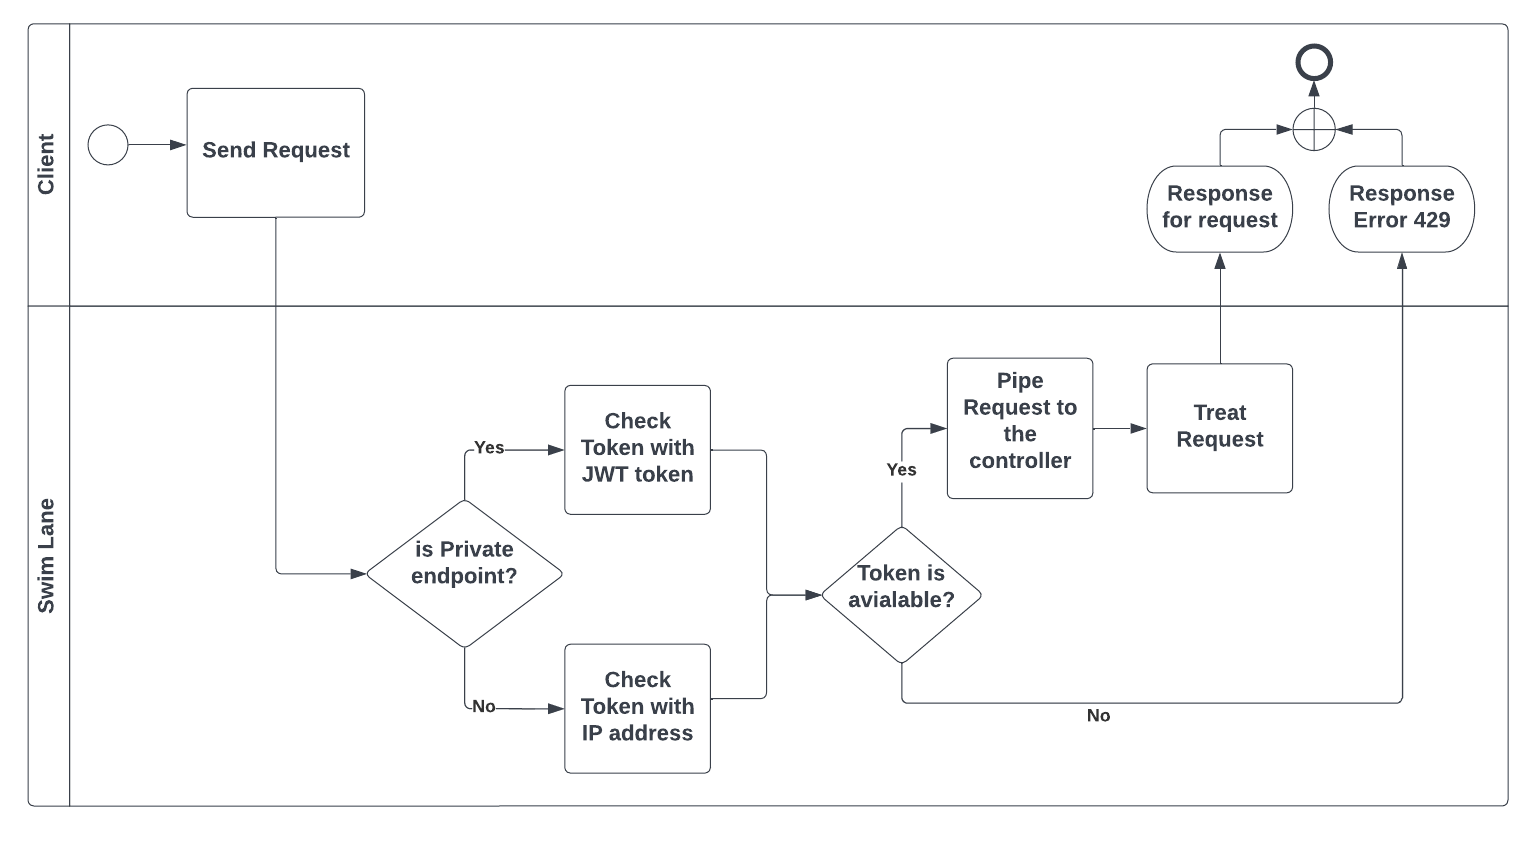
\includegraphics[width=\textwidth]{images/ratelimitingflow.png}
    \caption{\footnotesize{Rate Limiting Flow}}
    \label{fig:ratelimiting_flow}
\end{figure}

Rate limiting the user was specifically setup for handling the private endpoints and that
was able to be modified by the admin to allow for more or less requests per second
depending on the user, and the rate limiting the IP address was setup for the public API.

And lastly there was the rate limiting for the login, which was individually handled for
the purpose of limiting the number of login attempts per minute to avoid possibility
of a dictionnary attacks.

The testing of the rate limiting was done in a manual way, just to ensure that the ratelimiting 
indeed did block a real user.
And it was done using Httperf, which is a tool that allows to test the performance of a
web server. And as it could be used to generate requests and run them automatically,
it was used to overload the server over the threshold of the rate limiting.
The results of the tests displayed the following info:
\begin{itemize}
    \item The number of requests sent which was around 1100 and during the testing the threshold was around 1000.
    \item The number of requests receiving each type of response, so the number of requests that were with response code 100, 200, \dots
\end{itemize}

There were also other infos but that don't matter for the test case of rate limiting
as it was just to test the performance of the server. Which was not the aim of this.
And also we did a simple logging for reported ratelimit stopped requests just to make sure
the error were indeed rate limiting, and not some other error.

With this we had setup a good ground for rate limiting and for it's implementation
even if it required future updates on that part.
